\mysubsectionformatted{Diagrammi delle componenti e distribuzione}
\myparagraph{
    Sono diagrammi usati per poter raggruppare il codice in moduli e evitare le dipendenze tra loro (low coupling). Sono simili ai
    diagrammi delle classi, solo che invece di contenere le classi contengono rispettivamente i componenti e nodi.
    \\
    I \textbf{nodi} sono degli elementi fisici che possiedono memoria e capacità di elaborazione,
    vengono usati per modellare la tipologia dell'hardware, la distribuzione di componenti, sistemi client-server o un sistema
    embedded. Si possono raggruppare in package e all'interno di questi si possono specificare relazioni di dipendenza,
    generalizzazione, associazione e aggregazione.
    \\
    I \textbf{componenti} sono dei moduli di codice che partecipano all'esecuzione di un sistema, questi vengono eseguiti dai nodi
    (dato che esistono già a run-time). Come le classi, hanno un nome e possono realizzare più interfacce. Le componenti
    dispongono di operazioni raggiungibili solo attraverso le loro interfacce.\\
    \textbf{Ricorda\dots}
    \begin{itemize}
        \item Le \textbf{classi} sono \textbf{astrazioni logiche}.
        \item I \textbf{componenti} sono \textbf{oggetti fisici}, quindi l'implementazione delle classi.
    \end{itemize}
}

%DIAGRAMMA DELLE COMPONENTI
\mysubsectionformatted{Diagramma delle componenti}
\myparagraph{Come accennato prima, un componente è un modulo (o una parte modulare) di un sistema che incapsula i suoi contenuti rendendoli
    invisibli all'esterno (e quindi inaccessibili). I componenti possono essere sostituiti o aggiornati senza influenzare
    l'intero sistema, garantendo flessibilità e manutentibilità.
    \\
    I diagrammi delle componenti definiscono il comportamento delle interfacce fornite e richieste.
    \\
    L'obiettivo di questo diagramma è quello di enfatizzare l'importanza delle interfacce e di come i componenti siano
    vantaggiosi per i motivi spiegati sopra (indipendenza, modularità, riusabilità, rimpiazzabili senza influenzare il sistema...).
    \\
    I componenti possono definire sistemi software di dimensione e complessità arbitraria. I diagrammi UML delle componenti
    permettono di modellare i componenti software e le interfacce annesse.
    \\
    Si parla di \textbf{dipendenza (dependency)} tra due elementi quando alla modifica di uno dei due a sua volta
    potrebbe modificare anche l'elemento collegato.
    \\
    Spesso si fa riferimento a questo diagramma col nome di \textbf{Wiring Diagram}.
}

\newpage
\subsubsection{Esempio di diagramma delle componenti}
\begin{center}
    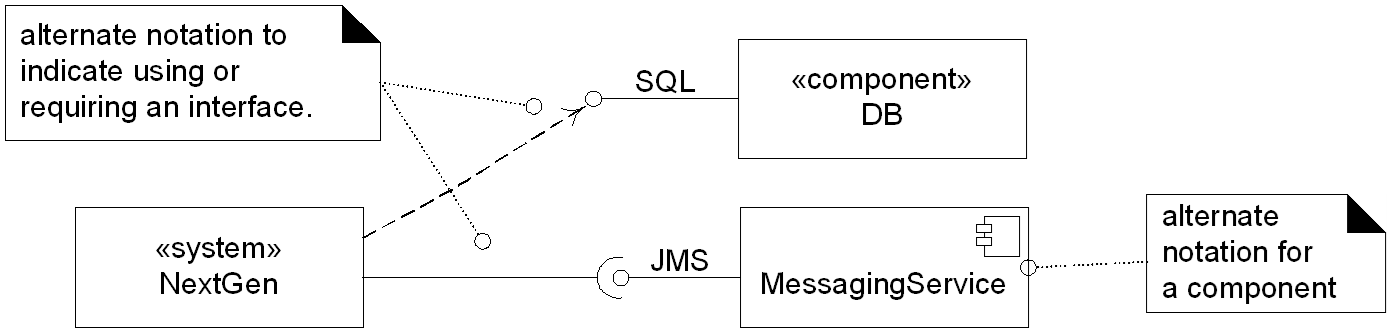
\includegraphics[scale=0.7]{diagramma_componenti/comp_diag_1.png}
\end{center}
\myparagraph{
    L'immagine sopra mostra come può essere dichiarato un componente in un diagramma UML, ovvero tramite notazione <<component>>
    oppure inserendo un simbolo sul lato destro.
    Altra cosa da ricordare è il collegamento tra il sistema e il componente, in base al tipo di freccia, indica se il componente
    sta \textbf{usando} (NextGen usa il DB) o \textbf{richiedendo} (NextGen richiede il MessagingService) \textbf{l'interfaccia}.
}

%DIAGRAMMA DI DISTRIBUZIONE
\mysubsectionformatted{Diagramma di distribuzione}
\myparagraph{
    I diagrammi di distribuzione (o deployment) mostrano l'assegnazione degli artefatti software concreti (es. file eseguibili)
    ai nodi computazionali (es. servizi di elaborazione).
    \\
    Mostrano la distribuzione degli elementi software all'interno dell'architettura fisica e la comunicazione tra questi.
    \\
    L'obiettivo di questo diagramma è quello di comunicare l'architettura fisica o di distribuzione.
}

\subsubsection{Elementi principali del diagramma di distribuzione}

\resizebox{\textwidth}{!}{
    \begin{tabular}{|l|l|}
        \hline
        \textbf{Nodo dispositivo}                 &
        \begin{tabular}[c]{@{}l@{}}Risorsa fisica con servizi di memoria e\\  processazione per eseguire il software.\end{tabular}                                                                                  \\ \hline
        \textbf{Nodo dell'ambiente di esecuzione} &
        \begin{tabular}[c]{@{}l@{}}Risorsa software che viene eseguita all'interno \\ di un nodo esterno (es. computer) e fornisce un servizio\\ per ospitare e eseguire un altro software eseguibile.\end{tabular} \\ \hline
        \textbf{Percorsi di comunicazione}        &
        Connessione tra i nodi.                                                                                                                                                                                     \\
        \hline
    \end{tabular}}

\myparagraph{
    Esempi di diagrammi di distribuzione posso essere degli artefatti, ovvero elementi fisici, come ad esempio \textbf{file eseguibili}
    (file JAR, .exe, script\dots) oppure \textbf{data files} (HTML, XML\dots).
    \\
    Un artefatto "\textbf{manifesta}" uno o più elementi di un modello. Con il termine manifestare si intende che l'artefatto rappresenta
    l'oggetto fisico di uno o più elementi del modello. Questi elementi solitamente sono dei componenti.
}

\newpage
\subsubsection{Esempio di uso di <<manifest>>}
Per rappresentare una manifestazione si usa una linea tratteggiata con freccia aperta etichettata con la keyword <<manifest>>

\begin{center}
    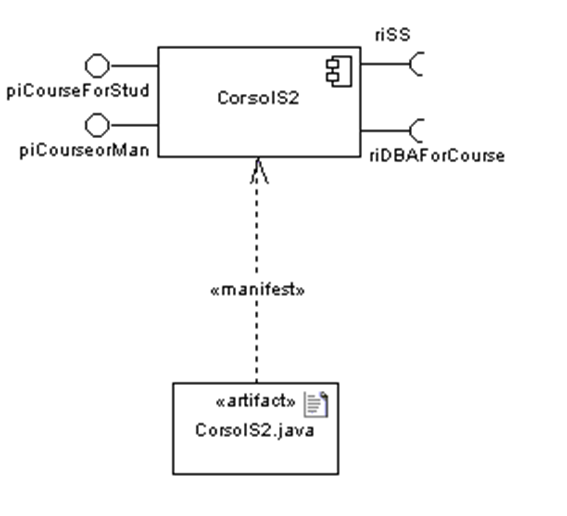
\includegraphics[scale=0.8]{img/diagramma_distribuzione/manifest_dg.png}
\end{center}

\mysubsectionformatted{CBSE, SOSE e Microservizi}
\myparagraph{
    In linea generale sono tre approcci all'ingegneria del software, ciascuno con diverse caratteristiche.
}

\mysubsectionformatted{CBSE - Component Based Software Engineering}
\myparagraph{
    Le parole chiave che determinano questo approccio sono la riusabilità e l'uso di componenti software.
    \\
    Questo approccio nasce dal momento che molto spesso lo sviluppo orientato agli oggetti fallisca per mancanza di riuso
    dei componenti, ciò è causato da vari motivi:

    \begin{enumerate}
        \item Le classi sono troppo dettagliate e specifiche per poter essere riutilizzate in altri contesti.
        \item I componenti sono più astratti delle classi stesse.
        \item I componenti vengono visti come dei provider di servizi indipendenti (stand alone).
        \item I componenti possono esistere come delle entità indipendenti.
    \end{enumerate}

    \newpage

    \noindent L'approccio CBSE fa sì che i componenti forniscano una funzionalità senza dover considerare dove il componente viene
    eseguito o il suo linguaggio di programmazione, questo perché è un'entità eseguibile e indipendente che può essere usato per
    uno o più oggetti eseguibili. L'interfaccia del componente è pubblica e tutte le interazioni avvengono tramite questa.
    \\
    Come per i diagrammi, questo approccio dispone di due tipi di interfacce:
    \vspace{-12pt}

    \begin{center}
        \resizebox{\textwidth}{!}{
            \begin{tabular}{|l|l|}
                \hline
                \textbf{Interfacce Fornite}   &
                \begin{tabular}[c]{@{}l@{}}Definiscono i servizi forniti dal componente verso altri componenti.\\ Essenzialmente, è l'API che definisce i metodi che possono essere chiamati dall'utente.\end{tabular}
                \\ \hline
                \textbf{Interfacce Richieste} &
                \begin{tabular}[c]{@{}l@{}}Definiscono i servizi richiesti dal componente per eseguire quanto specificato.\\ Ciò non compromette l'indipendenza o la distribuzione del componente perché l'interfaccia\\ richiesta non definisce come questi servizi vengono forniti.\end{tabular}
                \\ \hline
            \end{tabular}
        }
    \end{center}

    \vspace{8pt}

    \mysubsubsectionformatted{Componenti essenziali del CBSE}
    \begin{enumerate}
        \item Componenti indipendenti specificati dalle loro interfacce.
        \item Standard specifici dei componenti per facilitare la loro integrazione.\\
              Stabiliscono come i componenti comunicano e operano tra loro.
        \item Middleware che fornisce supporto per la portabilità dl componente.
        \item Un processo di sviluppo mirato al riuso.
    \end{enumerate}

    \mysubsubsectionformatted{Principi di progettazione}
    \begin{enumerate}
        \item I componenti sono indipendenti, non inteferiscono tra loro.
        \item L'implementazione dei componenti è nascosta.
        \item La comunicazione avviene tra interfacce ben definite.
        \item Le piattaforme dei componenti sono condivise in modo da ridurre i costi di sviluppo.
    \end{enumerate}

    I componenti sviluppati tramite diversi approcci NON lavorano tra loro.

    \mysubsubsectionformatted{Elementi basici di un modello di componente}
    \begin{center}
        \resizebox{\textwidth}{!}{%
            \begin{tabular}{|l|l|}
                \hline
                \textbf{Interfacce}    & \begin{tabular}[c]{@{}l@{}}Il modello dei componenti specifica come le interfacce devono essere definite\\ e i suoi elementi (operazioni, nomi, parametri...).\end{tabular}                                    \\ \hline
                \textbf{Uso}           & \begin{tabular}[c]{@{}l@{}}Per essere distribuiti e accessi in remoto, ciascun componente deve avere un\\ nome univoco.\end{tabular}                                                                           \\ \hline
                \textbf{Distribuzione} & \begin{tabular}[c]{@{}l@{}}Il modello dei componenti include una specifica di come i componenti \\ devono essere impacchettati per la loro distribuzione come entità\\ indipendenti e eseguibili.\end{tabular} \\ \hline
            \end{tabular}%
        }
    \end{center}

    \newpage
    \mysubsubsectionformatted{Processi del CBSE}
    I processi del CBSE sono, come dice il nome, dei processi software che supportano l'utilizzo di
    tale approccio. Permettono la riusabilità delle attività di processo coinvolte nelle attività
    di sviluppo e un riuso dei componenti.
    \\
    Bisogna fare una distinzione in merito alla modalità di sviluppo e il riuso:
    \vspace{-12pt}
    \begin{center}
        \resizebox{\textwidth}{!}{
            \begin{tabular}{|l|l|}
                \hline
                \textbf{Sviluppo PER il riuso} & \begin{tabular}[c]{@{}l@{}}Si basa sullo sviluppo di componenti che \\ verranno poi utilizzati in altre applicazioni.\end{tabular} \\ \hline
                \textbf{Sviluppo CON riuso}    & \begin{tabular}[c]{@{}l@{}}Si basa sullo sviluppo di nuove applicazioni\\ usando dei componenti già esistenti.\end{tabular}        \\ \hline
            \end{tabular}%
        }
    \end{center}
    \vspace{8pt}

    \mysubsubsectionformatted{Processi di supporto del CBSE}
    \begin{center}
        \resizebox{\textwidth}{!}{%
            \begin{tabular}{|l|l|}
                \hline
                \textbf{Acquisizione del componente}   & \begin{tabular}[c]{@{}l@{}}Processo che acquisisce i componenti per il loro riuso o trasforma\\ lo sviluppo in un componente riutilizzabile.\end{tabular}                        \\ \hline
                \textbf{Gestione del componente}       & \begin{tabular}[c]{@{}l@{}}Verte sulla gestione dei componenti riusabili assicurandosi\\ siano propriamente catalogati, immagazzinati e resi disponibili per il riuso.\end{tabular} \\ \hline
                \textbf{Certificazione del componente} & Processo che controlla se un componente soddisfa le sue specifiche.                                                                                                                 \\ \hline
            \end{tabular}%
        }
    \end{center}
    \vspace{8pt}

    \mysubsubsectionformatted{CBSE per il riuso}
    Si concentra sullo sviluppo dei componenti. Lo scopo è quello di generalizzare quei componenti che vengono creati per 
    specifiche applicazioni con lo scopo di renderli riutilizzabili.
    \\
    Un componente ha più probabilità di essere riutilizzato se è associato a un'astrazione di dominio stabile, ovvero a un oggetto
    di business ben definito e costante nel sistema.
    \\
    Per fare un esempio di dominio stabile può essere un ospedale, dove i componenti hanno ciascuno degli scopi fontamentali 
    (dottori, pazienti, trattamenti ecc\dots)

    \newpage
    \mysubsubsectionformatted{CBSE con riuso}
    Al contrario della prima tipologia, questa cerca e integra componenti già esistenti.
    Quando si riutilizzano i componenti in un progetto software, è fondamentale considerare i compromessi tra i requisiti ideali 
    di ciò che si desidererebbe avere e i servizi reali forniti dai componenti disponibili.
    \\
    Questo approccio richiede:
    \begin{enumerate}
        \item Sviluppo dei requisiti preliminari (essenziali).
        \item Ricerca dei componenti e la loro modifica in base alle funzionalità disponibili.
        \item Cercare nuovamente per trovare componenti migliori che soddifsano i requisiti.
        \item Unire (o comporre) i componenti per creare il sistema.
    \end{enumerate}

    \mysubsubsectionformatted{Problemi ancora aperti con CBSE}
    \begin{enumerate}
        \item Quanto è affidabile un componente senza un codice sorgente disponibile?
        \item Chi certifica la qualità dei componenti?
        \item Come possono essere predette le proprietà emergenti della composizione dei componenti?
        \item Come si fanno le analisi tra le caratteristiche di un componente con un altro?
    \end{enumerate}
}
    \newpage

\mysubsectionformatted{SOSE - Service Oriented Software Engineering}
\myparagraph{
    Le parole chiave che determinano questo approccio sono la riusabilità e l'uso di servizi software (per il CBSE era l'uso
    dei componenti software).
    \\
    Questo approccio nasce con lo scopo di fornire lo stesso servizio a più applicazioni o utenti, questo perché i servizi
    sono indipendenti tra loro.
    \\
    Per servizio si intende un'entità software con basso accoppiamento (loosely-coupled) che incapsula delle funzionalità che
    possono essere distribuite e accesse.

    \mysubsubsectionformatted{Standard di SOSE}
    \begin{center}
        \begin{tabularx}{\textwidth}{|>{\centering}m{2cm}|X|}
            \hline
            \textbf{SOAP} & Protocollo di accesso agli oggetti che definisce un'organizzazione per lo scambio di dati strutturati tra i web services.                                          \\ \hline
            \textbf{WSDL} & Definisce come possono essere rappresentate le interfacce dei web services.                                                                                        \\ \hline
            \textbf{UDDI} & Standard di ricerca che definisce come possono essere organizzate le informazioni di descrizione dei servizi, utilizzate dai richiedenti dei servizi per trovarli. \\ \hline
        \end{tabularx}
    \end{center}

    \subsubsection{Illustrazione dell'approccio SOSE}
    \begin{center}
        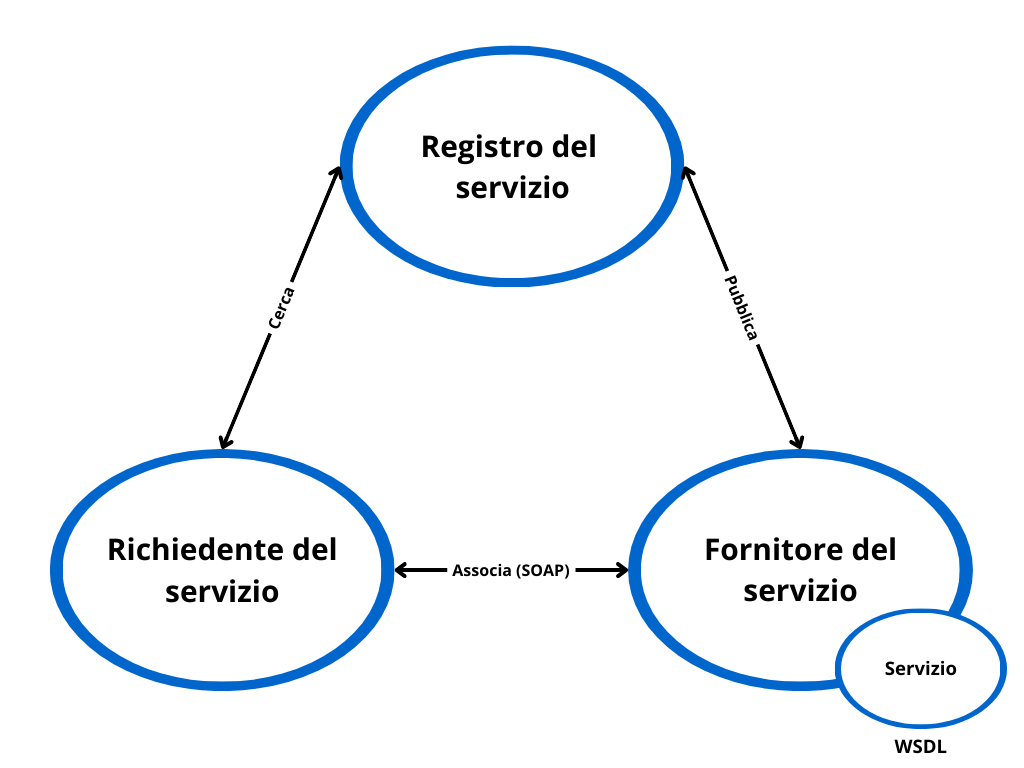
\includegraphics[width=10cm]{sose/funzionamento_sose.png}
    \end{center}
    \newpage

    \noindent Come per CBSE, anche SOSE distingue, nel suo caso, i servizi PER il riuso e i servizi CON riuso:
    \mysubsubsectionformatted{Servizi per il riuso}
    Come dice il titolo, questi servizi vengono sviluppati con lo scopo di essere riutilizzati all'interno di applicazioni orientati
    ai servizi. Questi servizi devono essere progettati come delle 'astrazioni riutilizzabili' che possono essere usati in sistemi diversi,
    in modo da poter garantire un servizio robusto e affidabile. Alla fine, il servizio deve essere ben documentato
    in modo da poter essere scoperto e capito da potenziali utenti.

    \mysubsubsectionformatted{Servizi con riuso}
    I servizi in questo caso vengono visti come dei componenti riutilizzabili. In questo modo, i servizi possono essere forniti localmente o
    esternamente verso altri fornitori. Altro vantaggio è che i servizi sono indipendenti dal linguaggio in cui vengono scritti, e per concludere
    l'investimento fatto in sistemi informatici obsoleti può essere preservato, conservandone quindi il valore attraverso aggiornamenti o
    modernizzazioni.

    \mysubsubsectionformatted{CBSE vs SOSE}
    La differenza sostanziale tra i due è che CBSE fa uso dei componenti, SOSE dei servizi.
    \begin{enumerate}
        \item I servizi sono indipendenti, i componenti no.
        \item I servizi non possiedono alcuna interfaccia 'richiesta'.
        \item La comunicazione tra i servizi avviene tramite messaggi in formato XML.
    \end{enumerate}
    \newpage
}

\mysubsectionformatted{MS - Microservices Software Engineering}
\myparagraph{
    Si tratta di uno stile architetturare che struttura l'applicazione come una\\ collezione
    di piccoli e contenuti componenti con basso accoppiamento. Questi componenti vengono anche
    chiamati servizi e implementano delle specifiche capacità di business.
    \\
    Tra le caratteristiche dei microservizi troviamo:
    \begin{enumerate}
        \item Comunicazione attraverso protocolli leggeri (lightweight).
        \item Sviluppati da team dedicati.
        \item La distribuzione è indipendente.
    \end{enumerate}
    L'obiettivo principale dei microservizi sarebbe quello di garantire scalabilità,\\ affidabilità, eterogeneità
    tecnologica e aggiornamenti continui del codice,\\ purtroppo, nella realtà ci troviamo di fronte a una
    complessa manutenibilità e una fase di testing difficile.

    \begin{center}
        \resizebox{\columnwidth}{!}{
            \begin{tabular}{c|c|c|}
                \cline{2-3}
                \multicolumn{1}{l|}{}                                                                                & \cellcolor[HTML]{3531FF}{\color[HTML]{FFFFFF} SOSE}                                                                                               & \cellcolor[HTML]{3531FF}{\color[HTML]{FFFFFF} MS}                                                                         \\ \hline
                \multicolumn{1}{|c|}{\textbf{Obiettivo}}                                                             & Riusabilità dei servizi                                                                                                                           & Garantire basso accoppiamento                                                                                             \\ \hline
                \multicolumn{1}{|c|}{\textbf{\begin{tabular}[c]{@{}c@{}}Di cosa\\ fa uso\end{tabular}}}              & \begin{tabular}[c]{@{}c@{}}Servizi: include tante funzionalità\\ di business e spesso è implementato\\ come un completo sottosistema\end{tabular} & \begin{tabular}[c]{@{}c@{}}Micro-servizi: creati per servire\\ solo una specifica funzionalità\\ di business\end{tabular} \\ \hline
                \multicolumn{1}{|c|}{\textbf{\begin{tabular}[c]{@{}c@{}}Cosa succede \\ alla modifica\end{tabular}}} & \begin{tabular}[c]{@{}c@{}}Richiede la modifica del sistema\\ monolitico, una modifica significativa\end{tabular}                                 & \begin{tabular}[c]{@{}c@{}}Richiede la creazione di un \\ nuovo servizio\end{tabular}                                     \\ \hline
                \multicolumn{1}{|c|}{\textbf{Comunicazione}}                                                         & Tramite ESB (Enterprise Service Bus)                                                                                                              & \begin{tabular}[c]{@{}c@{}}Meno elaborata e semplice \\ sistema di messaggi\end{tabular}                                  \\ \hline
                \multicolumn{1}{|c|}{\textbf{Protocolli}}                                                            & Multipli protocolli per messaggi (SOAP)                                                                                                           & Protocolli leggeri (HTTP, REST)                                                                                           \\ \hline
                \multicolumn{1}{|c|}{\textbf{Distribuzione}}                                                         & \begin{tabular}[c]{@{}c@{}}Uso di una piattaforma comune per\\ la distribuzione di tutti i servizi\end{tabular}                                   & \begin{tabular}[c]{@{}c@{}}Uso di una piattaforma cloud\\ per la distribuzione\end{tabular}                               \\ \hline
                \multicolumn{1}{|c|}{\textbf{Container}}                                                             & Uso poco popolare (Docker o Kubernates)                                                                                                           & Uso molto popolare                                                                                                        \\ \hline
                \multicolumn{1}{|c|}{\textbf{\begin{tabular}[c]{@{}c@{}}Archiviazione\\ dei dati\end{tabular}}}      & Condivisi tra i diversi servizi                                                                                                                   & \begin{tabular}[c]{@{}c@{}}Ogni micro-servizio può avere\\ un proprio archivio indipendente\end{tabular}                  \\ \hline
            \end{tabular}%
        }
    \end{center}
    \newpage
}

\mysubsectionformatted{Cloud Computing}
\myparagraph{
    Nasce per mano del NIST (National Instituite of Standard and Technology), si tratta
    di un modello capace di garantire un accesso via rete a una vasta area di risorse
    (reti, server, applicazioni, servizi ecc...) che possono essere rilasciate con la
    minima gestione o interazione con il fornitore del servizio.
    \\
    Tra le caratteristiche principali abbiamo:
    \begin{enumerate}
        \item Capacità per un utente di registrarsi e ricevere i servizi senza dover affrontare
              lunghe attese.
        \item Capacità di accedere ai servizi mediante piattaforme standard (desktop, laptop ecc\dots)
        \item Le risorse sono messe in comune tra tutti gli utenti o clienti.
        \item Scalabilità rapida per far fronte a un grande quantitativo di utenti.
        \item La fatturazione del servizio è monitorato in base a quanto si sta usando quel servizio.
    \end{enumerate}

    \mysubsubsectionformatted{La gerarchia del Cloud}
    \vspace{-1cm}
    \begin{center}
        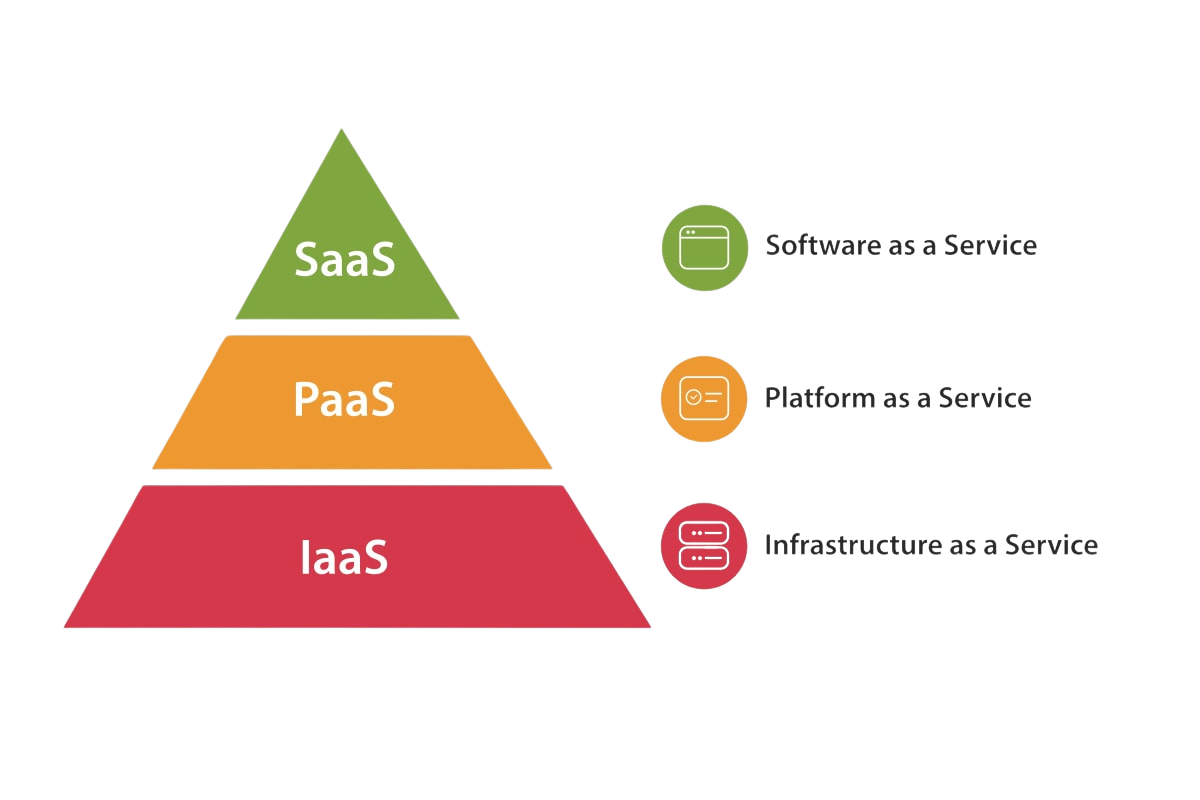
\includegraphics[width=13cm]{cloud/gerarchia_cloud.jpg}
    \end{center}

    \begin{center}
        \resizebox{\columnwidth}{!}{%
            \begin{tabular}{|l|l|}
                \hline
                \cellcolor[HTML]{009901}{\color[HTML]{FFFFFF} \textbf{SaaS}} & Applicazioni rivolte agli utenti finali, inviati tramite il web                                                                                  \\ \hline
                \cellcolor[HTML]{F56B00}{\color[HTML]{FFFFFF} \textbf{PaaS}} & \begin{tabular}[c]{@{}l@{}}Set di strumenti e servizi per creare codici e distribuire\\ le applicazioni in modo rapido e efficiente\end{tabular} \\ \hline
                \cellcolor[HTML]{CB0000}{\color[HTML]{FFFFFF} \textbf{IaaS}} & \begin{tabular}[c]{@{}l@{}}Hardware e software che da vita a tutti i servizi (server, \\ reti, sistemi operativi ecc\dots)\end{tabular}          \\ \hline
            \end{tabular}%
        }
    \end{center}
}